\chapter{Result From Flight Data}\label{ch:FlightResult}

This chapter is divided into three main sections. Firstly, the
algorithm's convergence and consistency was analyzed. Secondly, the
accuracy of the algorithm is examined by comparing to ground truth
data. The third section summarized test results for tuning the
algorithm for better accuracy and efficiency. The forth section
present the advantage of using IMU data. The fifth section outline
the inadequacies of the CC\_EKF\_SLAM algorithm identified.

To test the performace of CC\_EKF\_SLAM algorithm, 4 segments of video
were selected from the test flight video, and 400 frames were
processed in each piece. The filter initialized 40 features at the
first frame, and maintain the tracked features amount at this number
by initializing new features when existing features moved out of FOV.

Since all parameters are tracked in camera frame, their value is 
different when viewed from a fixed point in world frame. Therefore, all 
parameters are converted back to world frame before plotting. 

\section{Convergence and Consistency}

\subsection{Convergence and Tracking}
Among the feature parameters, the feature initialization point were
initialized to the zero which is the origin of the camera centric
coordinate. $\phi$ and $\theta$ were calculated directly from the
feature position on image plane, have high accuracy and don't require
convergence. The only parameter that goes through a converging process
is the features' inverse depth $\rho$, which were initialized to 0.1
for all features. Figure \ref{fltfig:1} shows the $1/\rho$ plot for
video segment1 over 200 frames. The depth estimators went through
rapid changes for several frames after their initialization. Within
approximate 20 frames, most estimtors settles to a stable value. The
estimated features distance ranged from 400 meters to about 1500
meters, confirming the algorithm's capability for estimating features
at great distance. On the other hands, some features take a long time
to settle, such as feature 9, 27, ??, while some other never settled,
such as 12 and 20.
% is the non and slowly settled feature has any character in its
% pattern? ie. is a line feature, instead of corner? A outlier filter
% should be in place to get rid of the poor features (future work).

\begin{figure}[h]
\centering
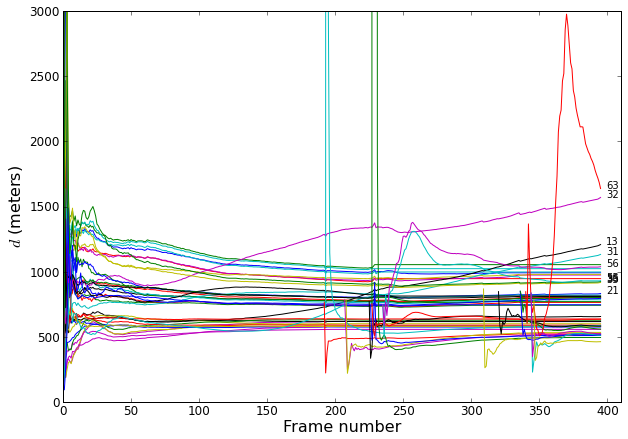
\includegraphics[width=10cm, keepaspectratio=true]{./Figures/fltfig/cut1/Figure10.png}
\caption{Inverse Depth Convergence}
\label{fltfig:1}
\end{figure}

Although the features initialization point $[x_i, y_i, z_i]$, and the
deviation-elevation angle pair $[\phi, \theta]$ did not go through a
converging stage, they do get updated and converted into the new
camera coordinate using the estimated camera motion at every
iteration. As a result, the accuracy of these parameters varies.
Ideally, the coordinates should converge to a fixed value. However,
the plot indicates a variation as the vehicle travels along. Figure
\ref{fltfig:2} shows the tracking of these parameters over 200 frames.
These parameters were stable for about 200 frames. Some features start
to drift after 200 frames. This coninside with the introduction of new
feature points into the system.
% are those featuers that drift are the one that's removed from the
% filter? 
% Does this prove that the filter altered the features parameter
% estimate in order to compensate for the incorrect estimate of the
% UAS localization. Since features removed from the filter were not
% altered for the comppensation, they shows a drift. 
 
% \begin{figure}[h]
% \centering
% 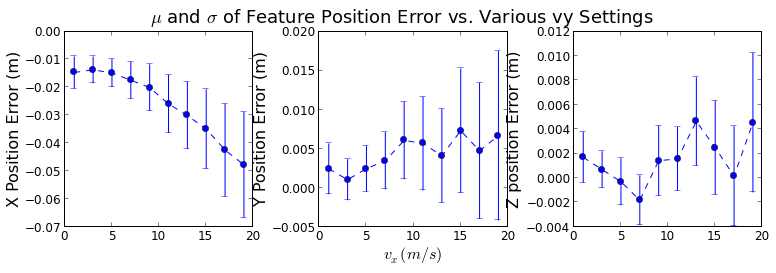
\includegraphics[width=12cm,keepaspectratio=true]{./Figures/fltfig/cut1/Figure20.jpg}
% \caption{Feature paramters (excluding $\rho$)}
% \label{fltfig:2}
% \end{figure}
\begin{figure}[h]
\centering
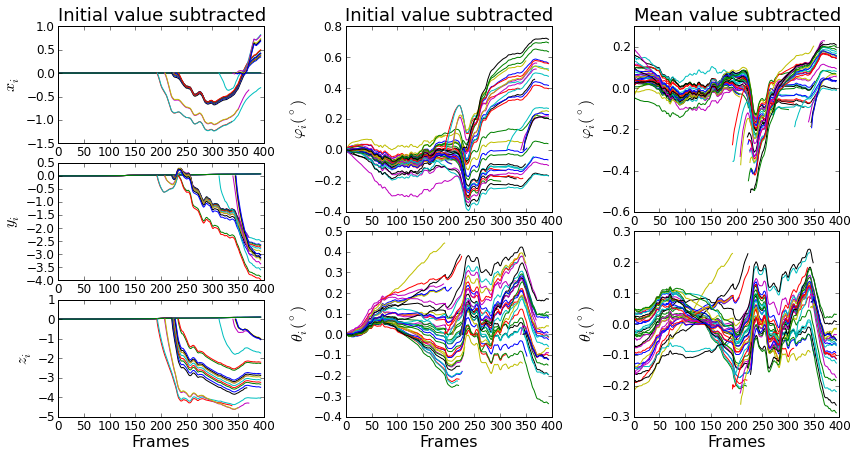
\includegraphics[width=10cm, keepaspectratio=true]
{./Figures/fltfig/cut1/Figure20.png}
\caption{Inverse Depth Convergence}
\label{fltfig:2}
\end{figure}
% is the drift still correlated with UAS? Stop plotting those features
% that's out of FOV to see what happen.
Comparing the pattern of the drift, it is highly 
correlated to the aircraft pitch and yaw rotation (figure?). The 
significant of the drift is measured by the maximum drift seen 
throughout the 200 processed frame, and are listed below (table?). The 
maximum drift is defined by:


%%% Local Variables:
%%% mode: latex
%%% TeX-master: "thesis"
%%% End:
